\begin{figure}
\centering	
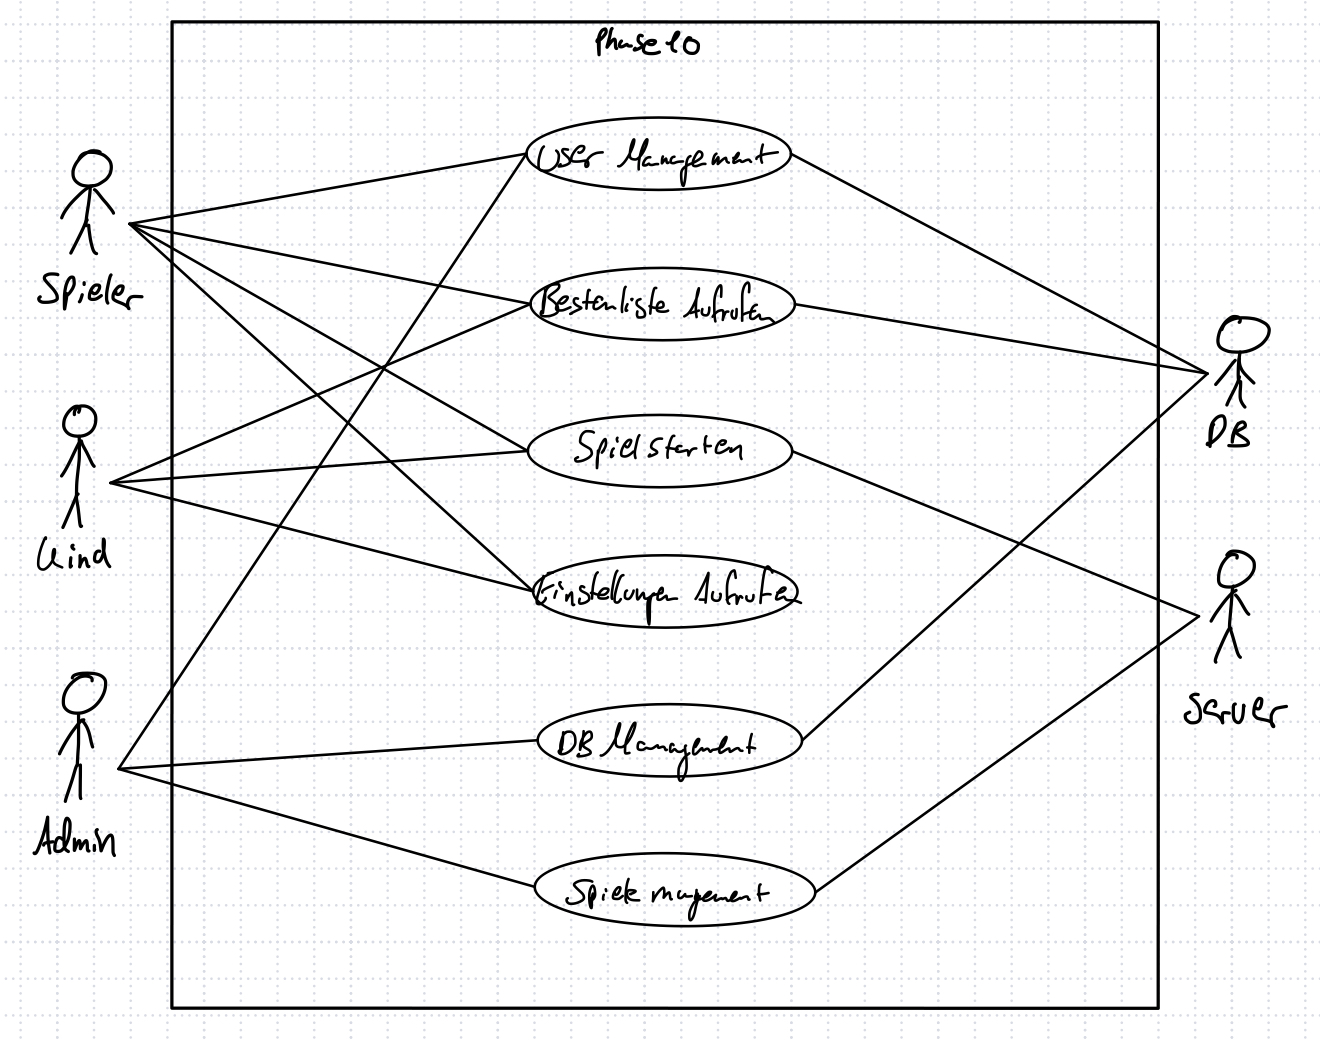
\includegraphics[width=0.9\textwidth]{img/use_case_diagram.jpeg}
\label{fig:sys}
\caption{Systemgrenzendiagramm (Use Case Diagramm)}
\end{figure}

\section{Systemgrenze (Use Case Diagramm)}

Die Systemgrenze wird in der Abbildung~\ref{fig:sys} dargestellt\footnote{Weitere Erklärungen und Spezifizierungen, die sich auf Abgrenzungen der Verantwortlichkeiten vom System und weiteren Akteuren/Systemen beziehen, können hier spezifiziert werden.}. 


\section{Beschreibungen der Anwendungsfälle}

Hinweis: Alle Systemfunktionen sind mit Anwendungsfällen zu decken! (Und dieser Hinweis ist zu löschen, wie auch der Beispielfall).

\newcounter{uc}\setcounter{uc}{10}

\begin{description}[leftmargin=5em, style=sameline]

	\begin{lhp}{uc}{UC}{uc:beispiel}
		\item [Name:] Name des Use Cases
		\item [Ziel:] Ziel und Zweck des Use Cases.
		\item [Akteure:] Akteure (auch benachbarte Systeme können Use Cases anfeuern), die den Use Case aktivieren können.
		\item [Vorbedingungen:] Eigenschaften des Systemzustands, in dem die Aktivierung des Use Cases möglich ist.
		\item [Eingabedaten:] Daten, die für die Ausführung des Use Cases nötig sind. Mit Referenzen auf~\ref{section:productdaten}.
		\item [Beschreibung:] Eine allgemeine Beschreibung des Use Cases.
		\item [Ausnahmen:] Verhalten des Systems in Ausnahmefällen (wenn etwas nicht ganz wie gedacht geht).
		\item [Ergebnisse und Outputdaten:] Beschreibung des Systemzustands nach einer erfolgreichen Ausführung des Use Cases sowie die auszugebenden Daten.
		\item [Systemfunktionen] Referenz auf die relevante(n) Systemfunktion(en).
	\end{lhp}

	\begin{lhp}{uc}{UC}{uc:usermanagement}
		\item [Name:] User Management
		\item [Ziel:] Verwaltung von Spieler Profilen
		\item [Akteure:] Spieler, Admin, DB
		\item [Vorbedingungen:] Spieler befindet sich auf der Hauptseite
		\item [Eingabedaten:] Zugriffsdaten ~\ref{daten:benutzername}~\ref{daten:passwort}~\ref{daten:kindersicherung}.
		\item [Beschreibung:] Spieler können hier ihren Account erstellen, bearbeiten, sich ausloggen oder ihren Account löschen. Bei der Erstellung eines Accounts kann angegeben werden, ob der Account ein Account mit Kindersicherung ist.
		\item [Ausnahmen:] Falls ein User einen Account erstellen möchte, den es bereits gibt, dann gibt das System eine Fehlermeldung an. 
		\item [Ergebnisse und Outputdaten:] Spieler ist auf der Hauptseite und sein Account ist erstellt/bearbeitet/gelöscht/ausgeloggt.
		\item [Systemfunktionen] \ref{funk:zugriff}
	\end{lhp}

	\begin{lhp}{uc}{UC}{uc:bestenlisteaufrufen}
		\item [Name:] Bestenliste aufrufen
		\item [Ziel:] Spieler kommen auf die Bestenlisteseite und können Highscores einsehen.
		\item [Akteure:] Spieler, Kind, DB
		\item [Vorbedingungen:] Spieler befindet sich auf der Hauptseite
		\item [Eingabedaten:] Keine Angaben benötigt
		\item [Beschreibung:] Spieler drückt auf einen Button und kommt auf die Bestenlisteseite. Auf der Bestenlisteseite wird die Anzahl der gewonnenen Spiele aller Spieler angezeigt.
		\item [Ausnahmen:] \begin{itemize}
						\item[] \textit{Datenbank fehler:} Das System zeigt eine Fehlermeldung an und der Spieler bleibt auf der Hauptseite.
						
					\end{itemize}
		\item [Ergebnisse und Outputdaten:]
		\item [Systemfunktionen] \ref{funk:bestenliste}
	\end{lhp}

	\begin{lhp}{uc}{UC}{uc:spielstarten}
		\item [Name:] Spiel starten
		\item [Ziel:] Starten eines Spiels
		\item [Akteure:] Spieler, Kind, Server
		\item [Vorbedingungen:] Spieler befindet sich auf der Hauptseite
		\item [Eingabedaten:] keine
		\item [Beschreibung:] Spieler können ein Spiel starten oder einem Spiel beitreten. Momentan offene Spiele werden in einem Serverbrowser aufgezählt.
		\item [Ausnahmen:] \begin{itemize}
			\item[] \textit{Server fehler:} Das System zeigt eine Fehlermeldung an und der Spieler bleibt auf der Hauptseite.
		\end{itemize}
		\item [Ergebnisse und Outputdaten:] Lobby ist erstellt und Spieler kommt in den Lobby-screen
		\item [Systemfunktionen] \ref{funk:spielraum}
	\end{lhp}
	
	\begin{lhp}{uc}{UC}{uc:dbmanagement}
		\item [Name:] Verwaltung der Datenbank
		\item [Ziel:] Admins können Daten direkt auf der Datenbank erstellen, einsehen, bearbeiten und löschen
		\item [Akteure:] Admin, DB
		\item [Vorbedingungen:] Datenbank gestartet
		\item [Eingabedaten:] keine
		\item [Beschreibung:] Direkter Zugriff auf Daten in der Datenbank. Daten können von Admins angelegt/verändert/gelöscht werden.
		\item [Ausnahmen:] \begin{itemize}
			\item[] \textit{Datenbank stürzt ab:} Admin hat somit keinen Zugriff mehr auf die Datenbankverwaltung, es können keine Änderungen mehr folgen.
		\end{itemize}
		\item [Ergebnisse und Outputdaten:] Beschreibung des Systemzustands nach einer erfolgreichen Ausführung des Use Cases sowie die auszugebenden Daten.
		\item [Systemfunktionen] Referenz auf die relevante(n) Systemfunktion(en).
	\end{lhp}

	\begin{lhp}{uc}{UC}{uc:spielmanagement}
		\item [Name:] Verwaltung von Spielen
		\item [Ziel:] Admins können Spiele starten und stoppen.
		\item [Akteure:] Admin, Server
		\item [Vorbedingungen:] Server gestartet
		\item [Eingabedaten:] keine
		\item [Beschreibung:] Admins können direkt auf dem Server Spiele verwalten.
		\item [Ausnahmen:] \begin{itemize}
			\item[] \textit{Server ist abgestürzt:} Admin hat somit keinen Zugriff mehr auf die Spielverwaltung, es können keine Änderungen mehr folgen.
		\end{itemize}
		\item [Ergebnisse und Outputdaten:] Spiele wurden gestartet/gestoppt.
		\item [Systemfunktionen] \ref{funk:spielverw}
	\end{lhp}

	% \begin{lhp}{uc}{UC}{uc:anmeld}
	% 	\item [Name:] Spieler anmelden.
	% 	\item [Ziel:] Spieler meldet sich im System an.
	% 	\item [Akteure:] Spieler.
	% 	\item [Vorbedingungen] Spieler ist im Vorraum.
	% 	\item [Eingabedaten:] Zugriffsdaten~\ref{daten:benutzername}~\ref{daten:passwort}.
	% 	\item [Beschreibung:] Spieler meldet sich an.
	% 	\item [Ausnahmen:] \hfill
	% 		\begin{itemize}
	% 			\item[] \textit{Passwort oder Benutzername ist falsch:} Das System zeigt eine Fehlermeldung an, anstatt des Schrittes 2.
				
	% 		\end{itemize}
	% 	\item [Ergebnisse und Outputdaten:] Spieler ist in der Lobby und sieht die Bestenliste.	
	% 	\item [Systemfunktionen:] \ref{funk:zugriff}.
	% \end{lhp}
	
	% \begin{lhp}{uc}{UC}{uc:anmeld}
	% 	\item [Name:] Spieler löschen.
	% 	\item [Ziel:] Spieler entfernt seine Daten aus dem System.
	% 	\item [Akteure:] Spieler.
	% 	\item [Vorbedingungen] Spieler ist im Vorraum.
	% 	\item [Eingabedaten:] Passwort~\ref{daten:passwort}.
	% 	\item [Beschreibung:] Spieler löscht das eigene Konto komplett.
	% 	\item [Ausnahmen:] \hfill
	% 		\begin{itemize} 
	% 			\item[] \textit{Passwort ist falsch:} Das System zeigt eine Fehlermeldung an, anstatt des Schrittes 2.
	% 			\item[] \textit{Keine Löschung erwünscht:} Anstatt des Schrittes 4, schließt das System den Dialog.
				
	% 		\end{itemize}
	% 	\item [Ergebnisse und Outputdaten:] Spieler ist im Vorraum, Spielerkonto wurde gelöscht.	
	% 	\item [Systemfunktionen:] \ref{funk:zugriff}.
	% \end{lhp}

\end{description}